\documentclass[Ex4_Zusammenfassung.tex]{subfiles}


\begin{document}

\section{Zerfallsbreite}
Wir wollen die Lebensdauer von kurzlebigen Teilchenzuständen (=Resonanzen: aus Stoßprozessen entstandene instabile Teilchen) herausfinden.\\

Der Zerfall eines instabilen Teilchens / einer Resonanz erfolgt nach dem Zerfallsgesetz:
\begin{equation}
	N(t) = N_0 \exp \lp - \lambda t \rp, \quad \lambda = \frac{1}{\tau}
\end{equation}

Der Zustand einer festen Energie $E_r$ ist durch die Wellenfunktion gegeben:
\begin{equation}
	\psi(t) = \underbrace{ \vphantom{\lp - \frac{i E_r t}{\hslash} \rp} \psi_0}_{\mathllap{\text{ortsabhängig}}} \cdot \underbrace{\exp \lp - \frac{\iota E_r t}{\hslash} \rp}_{\mathclap{\text{zeitabhängig}}}
\end{equation}

Die Wahrscheinlichkeitsdichte, ein Teilchen zu finden, ist:
\begin{equation}
	\psi^* \psi = \psi_0^2
\end{equation}
$\Rightarrow$ zeitlich konstant, kein Zerfall.\\
Dies führt uns zu dem Problem, dass sich auch für instabile Teilchen nur konstante Wahrscheinlichkeitsdichten ergeben.

\subsection*{Lösungsansatz}
Wähle komplexe Energie für zerfallende Teilchen:
\begin{equation}
	E = E_r - i \frac{\Gamma}{2}, \quad \Gamma \in \mathbb{R}
\end{equation}

Einsetzen in obige Gleichungen für Wellenfunktion und Wahrscheinlichkeitsdichte führt uns auf:
\begin{align}
	\psi(t) &= \psi_0 \exp \lp -i \frac{E_r t}{\hslash}\rp \exp \lp -\frac{\Gamma t}{2 \hslash} \rp\\
	\psi^* \psi &= \psi_0^2 \exp \lp -\frac{\Gamma t}{\hslash}  \rp
\end{align}
$\Rightarrow$ exponentieller Zerfall mit $\frac{\Gamma}{\hslash} = \lambda = \frac{1}{\tau};\ \Gamma \tau = \hslash$\\

Betrachte nun die Fourier--Transformierte der Wellenfunktion: $\psi(t) \stackrel{\mathcal{F}}{\Rightarrow} \psi(E)$:
\begin{align}
	\psi(E) &= \frac{1}{\sqrt{2 \pi}} \int_{0}^{\infty} \psi (t) \exp \lp i \frac{E t}{\hslash}  \rp \md t\\
	%%
	&= \frac{\psi_0}{\sqrt{2 \pi}} \int_{0}^{\infty} \exp \lp -t \lp \frac{i}{\hslash} \lp E_r  - E \rp + \frac{\Gamma}{2 \hslash} \rp \rp \md t \\
	%%
	&= \frac{\psi_0}{\sqrt{2 \pi}} \frac{i \hslash}{\lp E - E_r \rp + \frac{i \Gamma}{2}}
\end{align}

Daraus erhalten wir nun $P(E)$:
\begin{align}
	P(E) &= A \cdot \psi^*(E) \psi(E)\\
	\intertext{mit Normierung:}
	A &= \frac{\Gamma}{\hslash^2 \psi_0^2}
\end{align}

$P(E)$ heißt Lorentz-- oder Breit--Wigner--Verteilung. Ihr Maximum liegt bei $E_r$, ihre FWHM (= Full Width Half Maximum) bzw. Halbwertsbreite beträgt $\Gamma$.
\begin{equation}
	P(E) = \frac{\Gamma}{2 \pi} \frac{1}{\lp E - E_r  \rp^2 + \frac{\Gamma^2}{4}}
\end{equation}
\begin{figure}[H]
	\centering
	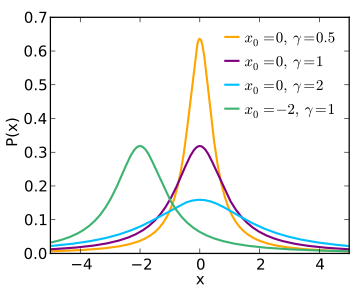
\includegraphics[scale=0.8]{Cauchy_pdf.png}
	\caption{Funktion für die Wahrscheinlichkeitsdichte der Lorentz--Verteilung}
\end{figure}

Aufgrund seiner endlichen Lebensdauer besitzt jedes Teilchen eine Energiebreite $\Gamma$. Über die Heisenberg'sche Energie--Zeit Unschärfe--Relation $\Delta t \Delta E \ge \nicefrac{\hslash}{2}$ ist die Lebensdauer eines instabilen Zustandes mit der Energieunschärfe verknüpft. Wird die Lebensdauer unmessbar klein $\rightarrow$ Zerfallsbreite $\Gamma = \frac{\hslash}{\tau}$, was eine messbare Größe ist.\\

$\Gamma$ und $\tau$ werden durch freigesetzte Energie (Phasenraum) und Art der Wechselwirkung bestimmt:
\begin{table}[H]
	\centering
	$
	\begin{array}{clrr}
		\text{WW} 	& \text{Teilchen} & \tau & \Gamma \\ \hline
		\text{stark} & \Delta (1232)     & 10^{-23} \si{s}& 100 \si{MeV}\\
		\text{el.mag.} & \pi^0 & 10^{-18} \si{s} & 1\si{keV}\\
		\text{schwach} & \pi^\pm & 10^{-8} \si{s} & 10^{-7}\si{eV}\\
		& n & 10^3 \si{s} & 10^{-18} \si{eV}
	\end{array} 
	$
	\caption{Übersicht einiger kurz- und langlebiger Teilchen(zustände). $\Delta(1232)$ ist ein Delta--Baryon (oder Delta-Resonanz) mit $m=1232 \si{MeV/c^2}$}
\end{table}

\end{document}